\chapter{Theoretical Background}
\label{cha:theoreticalBackground}
    %
    % MOLECULE DEFINITIONS -- START
        \definesubmol{lysine}{
            % 1
        R-[:330,0.7]\mcfbelow{N}{H}% 2
        -[:30,0.7]% 3
            (
        -[:330,0.7]% 4
                (
            =[:270,0.5]O% 6
                )
        -[:30,0.7]R'% 5
            )
            (
        <:[:50,0.7]H% 8
            )
        <[:110,0.7]% 7
        -[:30,0.7]% 9
        -[:330,0.7]% 10
        -[:30,0.7]% 11
        -[:330,.5,,1]NH_3^{\mcfplus}% 12
        }

        \definesubmol{acetylcoa}{
                % 1
            CoA-[:330,0.7]S% 2
            -[:30,0.7]% 3
                    (
                =[:90,0.5,,,red]{\color{red}O}% 5
                    )
            -[:330,0.7,,,red]% 4
        }

        \definesubmol{acetyllysine}{
                % 1
            R-[:330,0.7]\mcfbelow{N}{H}% 2
            -[:30,0.7]% 3
                    (
                -[:330,0.7]% 4
                        (
                    =[:270,0.5]O% 6
                        )
                -[:30,0.7]R'% 5
                    )
                    (
                <:[:50,0.7]H% 8
                    )
            <[:110,0.7]% 7
            -[:30,0.7]% 9
            -[:330,0.7]% 10
            -[:30,0.7]% 11
            -[:330,0.7]\mcfbelow{N}{H}% 12
            -[:30,0.7]% 13
                    (
                -[:330,0.7,,,red]% 15
                    )
            =[:90,0.7,,,red]{\color{red}O}% 14
        }
    % MOLECULE DEFINITIONS -- END
    %
    % \section{Epigenetics}
        % general and historic (very short or leave out)\\
        % instructive, responsive model\\
        % PCG Tri\\
    %
    %
    \section{Eukaryotic transcription regulation}
        %
        \subsection{Chromatin}
            %
            Eukaryotic DNA is organized as chromatin in the cell nucleus, which consists of nucleosomes that mainly serve the increase of packing density and robustness of the DNA, but also plays an important role in gene regulation. Nucleosomes are built out of DNA wrapped around an octamer of homologous, basic proteins, the histones. These proteins contain a great amount of the positively charged amino acids arginine (Arg, R) and lysine (Lys, K), which results in attracting the negatively charged DNA (phosphate backbone). The so-called histone tails on the amino end of the proteins stick out of the nucleosome core complex. Albeit not having a fixed secondary structure, the tails, as well as the rest of the histones are very well conserved throughout a large set of eukaryotes, from \textit{Saccharomyces cerivisiae} all the way to \textit{Homo Sapiens Sapiens} \cite{berg2015stryer}.\\ %TODO Image from Xd with schematic nucleosome explaining linker DNA, Octamer (Dimers and Tetramer?) H1, etc. Add "inspired from..."
            %
            \begin{figure}[htpb!]
                \centering
                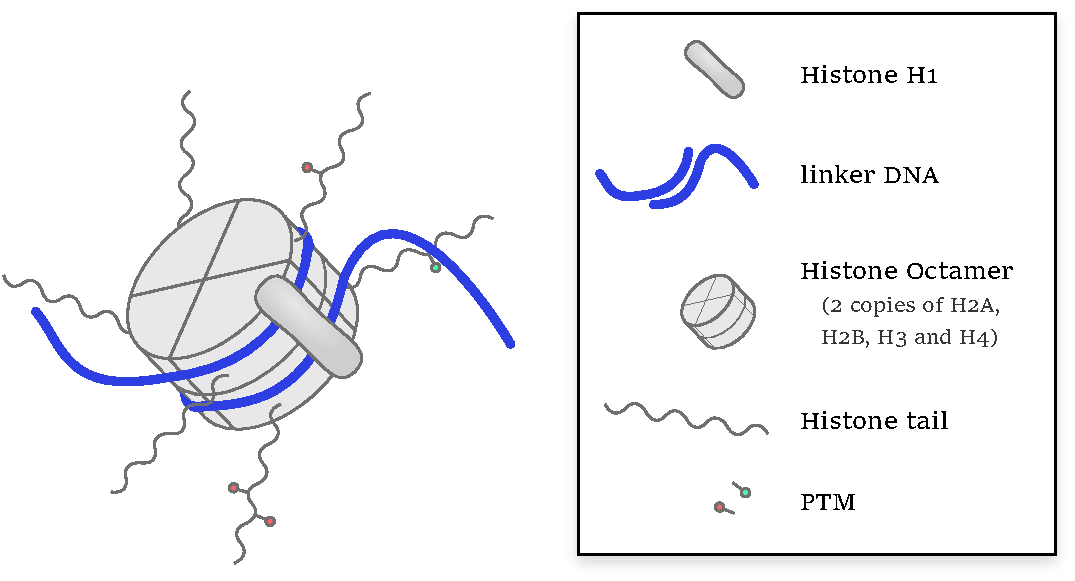
\includegraphics[width=0.7\textwidth]{annotated_nucleosome.pdf}
                \caption{schematic model of a nucleosome} % TODO complete caption.
                \label{img:nucleosome}
            \end{figure}
            %
            Chromatin can show higher order structure than the simple “beads on a string” variant. As such, nucleosomes that are not necessarily next neighbours along the DNA string can be in near proximity \cite{berg2015stryer, }.\\ % TODO The following higher order structures have been found by... % FIXME Source
            %
            Chromatin structure plays an important role in eukaryotic gene expression. Some DNA segments close to and on an actively transcribed gene are more easily accessible by proteins due to a locally more open chromatin structure. These chromatin regions are therefore called hypersensitive sites. \cite{cooper2017genome} Logically, the location of hypersensitive sites depends on the set of active genes and is thus cell-type and age specific \cite{berg2015stryer}.\\
            %
            The complex process of chromatin remodelling which leads to activation or repression of gene transcription comprises a vast multitude of agents and their interaction network is still not fully understood.\\
            %
        %
        %
        \subsection{Histone-modifying enzymes}
            %
            This thesis is based on one aspect of the chromatin remodelling machinery, namely histone-modifying enzyme complexes (HME). These complexes are able to covalently bind or remove chemical groups on amino acids (mostly R and K) at specific positions on the histone tail. The presence of these chemical groups changes the charge or polarity of the modified amino acids and thus influence the histone's affinity to the DNA. Histone-acetyltransferases (HATs), for instance, add an acetyl group to lysine, thus neutralizing the positive charge on the ammonium cation at neutral pH (see figure \ref{img:acetyllysineReaction}). This neutralization decreases the attraction to the negatively charged DNA backbone significantly resulting in the occurrence of a hypersensitive site. \cite{berg2015stryer} \\
            %
            \begin{figure}[htpb]
                \centering
                \vspace{.5cm}
                \schemestart
                    \arrow{0}[,0]
                    \chemname{\chemfig{!{lysine}}}{Lysine}\+\chemname{\chemfig{!{acetylcoa}}}{Acetyl-CoA} % TODO paint the acetyl-group red
                    \arrow[-90]
                    \chemfig{!{acetyllysine}}\+\chemfig{CoA-SH}\+\chemfig{H^+}
                \schemestop
                \vspace{.5cm}
                \caption{Acetylation of lysine. This reaction is catalysed by the HAT enzyme which by means of the cofactor acetyl coenzyme A (Acetyl-CoA) is able to trigger the transfer (substitution reaction in chemical terms) of an acetyl group onto the nitrogen atom in the side chain of lysine. The latter can be part of a histone tail.}
                \label{img:acetyllysineReaction}
            \end{figure}
            %
            Apart from the acetyl group, a multitude of other markers have been found on histone tails, e.g. methylation (one-, two and three-fold), phosphorylation, ubiquitylation, etc. These groups can entail gene transcription activation, silencing (repressing), or completely different purposes.\\ % FIXME source
            %
            This thesis will only feature acetylation as an activating modification and methylation as a silencing modification. Accordingly, the “state” of a nucleosome is defined as one of the following:
            %
            \begin{itemize}
                \item \textbf{unmodified}: There has been no PTM on any histone tail of the concerning nucleosome.
                \item \textbf{active}: Every PTM found on the concerning nucleosome enables gene activation. In this thesis, every one of these PTMs is an acetylation.
                \item \textbf{silent}: Every PTM found on the concerning nucleosome disables gene activation. In this thesis, every one of these PTMs is a methylation.
                \item \textbf{bivalent}: see \ref{sec:bivalency}
            \end{itemize}
            %
        %
        %
        \subsection{Bivalency}
            %
            \label{sec:bivalency}
            In pluripotent stem cells, nucleosomes have been found to contain both activating and silencing markers on histone tails of one and the same octamer. This bivalent state is believed to maintain a “poised state”, being ready to induce a gene expression cascade as soon as the silencing marker is removed. % FIXME source
            Others believe, that this bivalent state is connected to cell division and the ability of inheriting the active gene set for one daughter cell to induce differentiation while the other daughter cell remains a pluripotent stem cell \cite{schuettengruber2017genome}. % TODO is this right?
            %
            % TODO maybe add important enzyme types from biology here to later refer to them when explaining the models in ED
            %
        %
        %
    %
    %
    \section{Dynamic histone PTM models}
        %
        \subsection{(Solving the) chemical master equation}
            %
            The chemical master equation (CME) is the differential equation underlying the system that describes the time-dependent evolution of that system from a reactive point of view. Applied to the case at hand, we can establish the CME system made out of two equations for either the concentration of active (acetylated) and silent (methylated) nucleosome states.\\
            %
            In order to do this, one can establish the Langevin stochastic differential equation \cite{lemons1908paper} for each HME type, as was already done by Mayer in \cite{mayer2020langevin}. % TODO Langevin or CME?
            Eq. \ref{eqn:noncooperative} describe the noncooperative (see % TODO where do I explain cooperative?
            ) case for $a = \frac{A}{N}$ and $m = \frac{M}{N}$ with $A$ the number of acetylated nucleosomes, $M$ the number of acetylated nucleosomes and $N$ the total number of nucleosomes. $\alpha_i$ and $\beta_i$ are coefficients taking into account the types, association and dissociation ratios of the enzymes in the system.\\
            %
            \begin{subequations}
                \begin{align}
                    &\frac{\partial a}{\partial t} = \underbrace{- \alpha_1 a }_{\textrm{ac removal}} + \underbrace{ \alpha_2 a*(1-a-m) }_{\textrm{ac addition}}\\
                    &\frac{\partial m}{\partial t} = \underbrace{- \beta_1 m }_{\textrm{me removal}} + \underbrace{ \beta_2 m*(1-a-m) }_{\textrm{me addition}}
                \end{align}
                \label{eqn:noncooperative}
            \end{subequations}
            %
            Obviously, this would only be a usable model if the neighbour relations of the nucleosomes can be neglected. Given that the context from the enzyme rule sets is an important aspect of EpiDynast, an analytical solution of the CME would not be the best approximation. Also, depending on discrete numbers such as the number of nucleosomes in the string, the analytical solution of the CME as a continuous system, makes it even more unfitting as an approximation.\\
            %
            A more fitting system would be to establish and solve the CME for every nucleosome while the CME for nucleosome $i$ would depend on the number of neighbours equal to the biggest enzyme context in the system. So, if the rule set contains at least one rule including the next neighbours of the modified nucleosome $i$, the CME system would change to eqn. \ref{eqn:neighbourDependent}
            %
            \begin{subequations}
                \begin{align}
                    &\frac{\partial a_i}{\partial t} = - \alpha_1 (a_{i-1} + a_i + a_{i+1}) + \alpha_2 (a_{i-1} + a_i + a_{i+1})*(1-a-m)\\
                    &\frac{\partial m_i}{\partial t} = - \beta_1 (m_{i-1} + m_i + m_{i+1}) + \beta_2 (m_{i-1} + m_i + m_{i+1})*(1-a-m)
                \end{align}
                \label{eqn:neighbourDependent}
            \end{subequations}
            %
        %
        %
        \subsection{Gillespie's algorithm}
            %
            Gillespie's algorithm simulates the time evolution of a spatially homogenous molecular mixture under specification of the coupled reaction channels (i.e. association and enzymatic reaction with dissociation) based on stochastic chemical kinetics \cite{gillespie1976general, gillespie1992rigorous}. This is useful especially when solving the chemical master equation analytically is not ideal.\\
            %
            \begin{itemize}
                {
                    \color{red}
                    \item next-neighbours
                    \item rule-based, (paper from Arnold, Prohaska is basis for Nico's work, also basis for my work)
                    \item Gillespie's
                        \begin{itemize}
                            \item explain event based
                            \item steps from his paper
                        \end{itemize}
                    \item association and concentration are taken together.
                    \item enzyme types

                }
            \end{itemize}
            %
        %
        %
        \subsection{EpiDynast}
            %
            The software used in this thesis is \ed, developed by Herbig et al. % FIXME source for EpiDynast
            The main working mechanism may be outlined as follows: After defining enzyme rule sets and a starting nucleosome string (concerning their PTMs %TODO are these PTMs? DId I explain PTM?
            ), \ed simulates the stochastic time-dependent change of said modifications on the string, exactly one event at a time. The two events that can occur for each enzyme are either an association step or a reaction step that immediately entails dissociation of the enzyme from the nucleosome.\\
            %
            The enzyme rule sets simply describe a pattern (further on called “context” % TODO is the context including the site that is changed?
            ) on the string, that is then changed according to the rule. For instance, a linear acetylation extender enzyme % TODO either reference or put a picture
            would look for a pattern with two neighbouring nucleosomes, one acetylated and the other one unmodified and acetylate the latter.\\
            %
        %
        %

    %
    %
    \section{Epigenetic fitness landscapes} % TODO change title
        %
        \subsection{From landscape to vector field}
            %
            The term of epigenetic fitness landscape (referred to as landscape in the rest of this thesis) is mathematically defined as the triple $(V, \chi, f)$ where $V$ is a set of configurations, $\chi$ refers to the neighbouring relationship or similarity among the configurations and $f$ defines the fitness function of the landscape.\\ % FIXME source stadler
            %
            In this case, $V$ comprises the entirety of active, silent and unmodified state distributions along the nucleosome string, $\chi$ determines the modification of one nucleosome state, e.g. from silent to unmodified, or vice versa and $f$, which indicates the relative height or depth $f(v)$ of a specific configuration $v \in V$, is determined by all the association and dissociation rates, as well as the type of the enzymes in the system. In this specific landscape, the stochastic Gillespie's algorithm will always tend towards configurations (fix points) at the very base of landscape basins. These configurations are those, that are adopted in the majority of time steps throughout Gillespie's algorithm simulation.\\
            %
            \begin{figure}[htpb!]
                \centering
                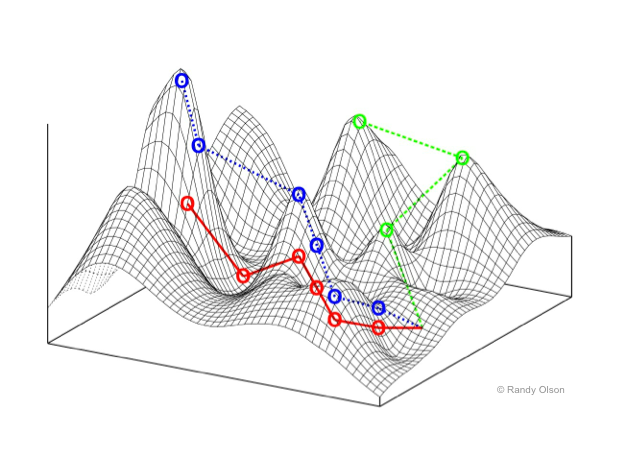
\includegraphics[width=0.7\textwidth]{prov_fitnessLandscape.png}
                \caption{Fitness landscape example and 2D projection.} % TODO change image to a self-made one. Maybe more intuitively usable for the case at hand
                % TODO insert tails and PTMs
                \label{img:fitnessLandscape}
            \end{figure}
            %
            Depending on the landscape, e.g. if there are deep and steep basins, it gets more and more difficult for the stochastic algorithm to exit the basin and adopt a configuration that lies outside. Each histone modifying enzyme thus induces a stability trend among the configurations which results in a vector field specific to each type of enzyme. In more complex systems with a multitude of different enzymes, these vector fields are combined % TODO no simple sum
            and create the resulting landscape at hand containing one or more fix points.\\
            %
            In this thesis,  there won't be any numerical values given to $f(v)$. However, by modifying the relative enzyme rate ratios, one can easily see that $f$ can change drastically resulting in it being much harder for the system to maintain a certain state or move along the shape of the landscape to switch from one state to another.\\ % TODO move this to discussion
            %
        %
        %
        \subsection{Enzyme types and bistability}
            %
            The number of fix points in the landscape can be analytically derived from the enzymes and their dependence on the frequency of nucleosome states (e.g. acetylation, methylation, ...) over time (see eqns. \ref{eqn:noncooperative}).\\
            %
            Mayer solved the equations analytically and found 4 critical values \cite{mayer2020langevin}: 3 fix points at $(0,0)$, $(0,1-\frac{\beta_1}{\beta_2})$, $(1-\frac{\alpha_1}{\alpha_2},0)$ and a separatrix that depends on the ratio between $\frac{\alpha_1}{\alpha_2}$ and $\frac{\beta_1}{\beta_2}$. The separatrix always has a gradient towards one of the non-trivial fix points. If $\frac{\alpha_1}{\alpha_2} = \frac{\beta_1}{\beta_2}$, the separatrix has no gradient.\\
            %
            \begin{figure}[ht!] % TODO include captions for vector graphs
                \centering
                \begin{minipage}{0.3\textwidth}
                    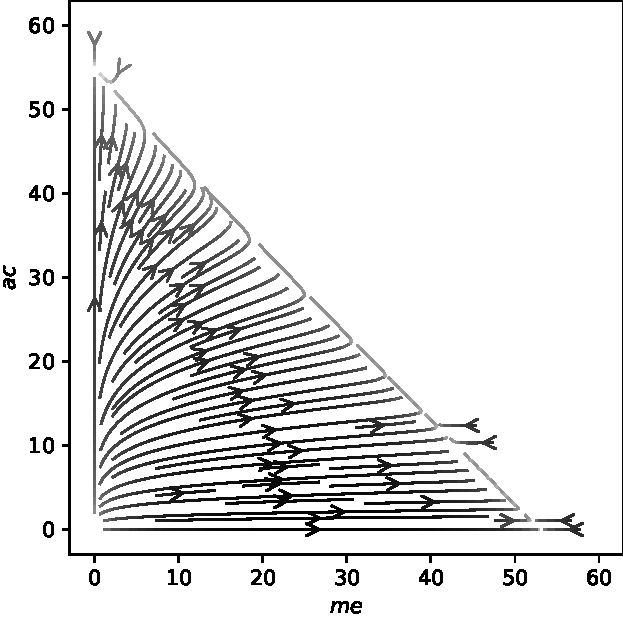
\includegraphics[width=\textwidth]{vectorfield_noncooperative_assymetric_monostable_ac.pdf}
                    \caption*{\small \textbf{(a)}}
                    \label{}
                \end{minipage}
                \begin{minipage}{0.3\textwidth}
                    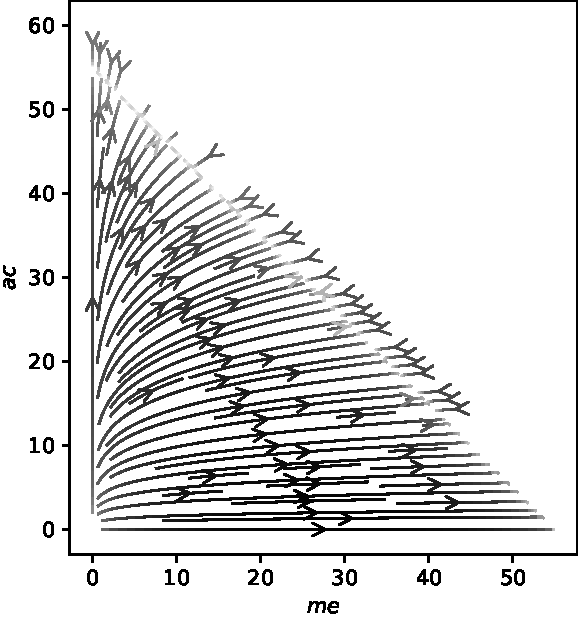
\includegraphics[width=\textwidth]{vectorfield_noncooperative_asymmetric_multistable.pdf}
                    \caption*{\small \textbf{(b)}}
                    \label{}
                \end{minipage}
                \begin{minipage}{0.3\textwidth}
                    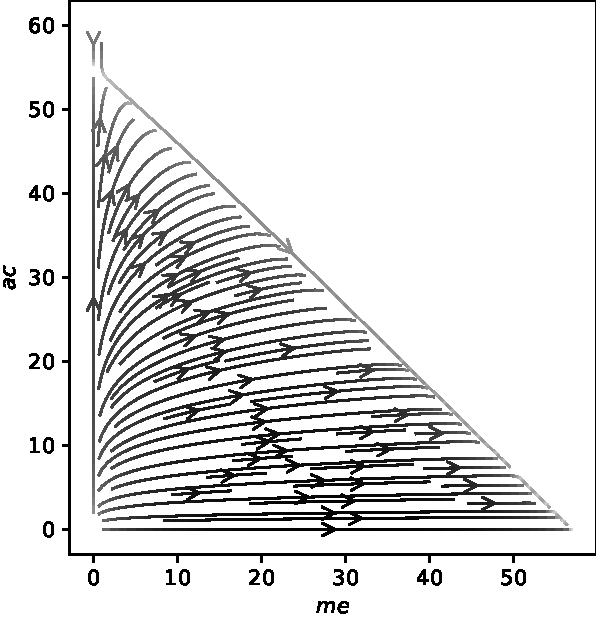
\includegraphics[width=\textwidth]{vectorfield_noncooperative_assymetric_monostable_me.pdf}
                    \caption*{\small \textbf{(c)}}
                    \label{}
                \end{minipage}
               \caption{\small  intervals.}
            \end{figure}
            %
            \begin{itemize}
                {
                    \color{red}
                    \item Can it be shown that the separatrix is only zero gradient if there is a null vector field?
                }
            \end{itemize} % TODO Can it be shown that the separatrix is only zero gradient if there is a null vector field?
            %
            In order for a dynamic histone PTM system to be bistable, the enzymes have to show cooperativity \cite{dodd2011barriers,sneppen2019theoretical,mayer2020langevin}. According to Sneppen \cite[][p.48]{sneppen2014models}, \enquote{cooperative binding means that the probability of occupying a state increases more than linearly with the concentrations of the binding molecules}.\\
            %
            In \cite{dodd2011barriers}, Dodd et al. specify the nature of cooperativity in order to reach ultrasensitivity\footnote{From Dodd et al. \cite{dodd2011barriers}: \enquote{Ultrasensitivity is a nonlinearity that magnifies any numerical advantage of one nucleosome type over another, allowing positive feedback to strongly push the system away from intermediate states and towards a large majority of one or other type.}} and thus a bistable system as follows\footnote{citations inside the quote changed their appearance in order to remain functional and to stylistically fit this work}:
            %
            \begin{quote}
                “Cooperativity can be direct, where two modified nucleosomes act together to recruit an enzyme to modify a third nucleosome \cite{3dodd2007theoretical,11sedighi2007epigenetic,15micheelsen2010theory}, or indirect, where each modified nucleosome catalyzes one of two separate modification reactions to fully convert a third nucleosome \cite{3dodd2007theoretical,13david2009inheritance}. A critical requirement for ultrasensitivity is that modified nucleosomes must act nonlocally, stimulating modification of nucleosomes located some distance away on the DNA. This long-range interaction is necessary for any nucleosome to be able to ‘sense’ the majority nucleosome type within the patch and cannot be provided by simple neighbor-to-neighbor contact \cite{3dodd2007theoretical,15micheelsen2010theory}.”
            \end{quote}
            %
            In other words, cooperativity can only be achieved by allowing the enzymes to detect more than one nucleosome that, in order to reach bistability, must not be a direct neighbour of the nucleosome to be (un)modified. This allows the modification that is superiorly prevalent over the whole string at that moment to be accounted for and recognized by the enzymes.\\
            %
            On a sidenote, the definition of cooperativity might seem slightly counterintuitive from a biochemical point of view, where the notion of cooperativity is strongly associated to be an asset of the enzyme \cite{cooperativityDefBritannica}. In contrast, according to Dodd et al., cooperativity is described as being a property of a set of nucleosomes being able to “cooperate” in order to recruit an enzyme and catalyse a reaction. Even though this not ideally put from a biochemical point of view, the mathematical implications still remain valid.\\ % TODO rephrase the notion of cooperativity from biochemical point of view
            %
            \begin{itemize}
                {
                    \color{red}
                    \item rephrase the biochemical side of cooperativity?
                }
            \end{itemize}
            %
            Mayer in \cite{mayer2020langevin} expressed the time dependent concentration of the modifications in the system in function of cooperative enzymes in the following differential equation system:
            %
            \begin{subequations}
                \begin{align}
                    &\frac{\partial a}{\partial t} = \underbrace{- \alpha_1 a }_{\textrm{ac rem}} + \underbrace{ \alpha_2 \frac{1}{n} a^2*(n-a-m) }_{\textrm{ac add}}\\
                    &\frac{\partial m}{\partial t} = \underbrace{- \beta_1 m }_{\textrm{me rem}} + \underbrace{ \beta_2 \frac{1}{n} m^2*(n-a-m) }_{\textrm{me add}}
                \end{align}
                \label{eqn:cooperative}
            \end{subequations}
            %
        %
        % TODO include Matilda's vector graphs
        \begin{itemize}
            {
                \color{red}
                \item Include Matilda's vector graphs
                    \begin{itemize}
                        \item Mark the fix points and separatrix
                    \end{itemize}
            }
        \end{itemize}
        %
    %
    %
    \section{Transition}
        %
        Although the mathematical foundation on whether a system can and cannot show bistability was already established, the execution in terms of building a model and rigorously identifying the influence of different factors within the model on the dynamics of a bistable system have, to my knowledge, not been explored yet.\\
        %
        Also, to date, bistable systems have not yet been modelled by means of a software that takes limited enzyme reach into account like \ed does.\\ % TODO remove space behind ED
        %
        This thesis will show exactly that. % TODO change sentence
        %
    %
    %
%
%
